\chapter{Results and discussion}
\label{chap:results}
In this chapter, the findings made in the thesis are presented. This chapter mostly consists of a discussion of why there is a difference in certain cloud and radiation variables between the run with removed sea ice and the control run, and the run with increased aerosol number concentration and the control run. At the end, there is also a small section on the difference from the control run when both the sea ice is removed and the aerosol number concentration is increased.

The results are discussed separately for removed sea ice and increased aerosol number concentration and for days 1 and 5. Where day 1 represents the closest to an "off line" run, whereas by day 5 the atmosphere has had some time to adjust to the changes.

I also try to answer if these results show a warming or cooling effect and if there is reason to believe that changes in sea ice extent and aerosol concentration will further influence the sea ice extent.

The discussion is based on differences in daily averages for the fields. The daily averaged differences have been calculated by subtracting the field from the control run for one time from the same field at the same time from a different run, these differences have then been added together and divided by the number of differences that were added together.(@ insert equation for clarity?)

But first, to have a reference for the differences, the weather and cloud situation for the control run is presented.

%--------------------
\section{Reference figures from the control run}
%--------------------
Figure~\ref{fig:weather} shows the weather situation in the control run for days 1 and 5. The temperature at 2~m height is represented by red contour lines, and the wind speed and direction at 10~m height is shown by the 
wind barbs and their color. Day 1, figure~\ref{subfig:weather_cont_day1} shows weak northerly winds ($\sim$ 5~m/s) bringing cold air (@ input temperature) from the north over the sea ice, and the westerly winds over the ocean south of the sea ice bring moisture to the air over the sea ice which is seen as low stratus in figure (@subfig cross section), which shows the LWC in the vertical cross section over the red line in figure (@ref line cross). The thicker clouds over the island in figure (@subfig cross section) have been formed due to orographic lifting. The westerly winds over the sea ice towards the mountains at $\sim$76$\degree$N and 112$\degree$W has brought the air to saturation as it is lifted and formed thick clouds over the mountains with LWC of $\sim$@(input value from cross section). From figure (@subfig ice cross), showing the ice water content (IWC) in the section one can see that the thicker clouds over the mountain also contains ice in the upper part of the clouds, with about @(input value)~$\text{mg/m}^{-3}$. 

\begin{figure}
    \centering
    \begin{subfigure}{0.48\textwidth}
        \centering
        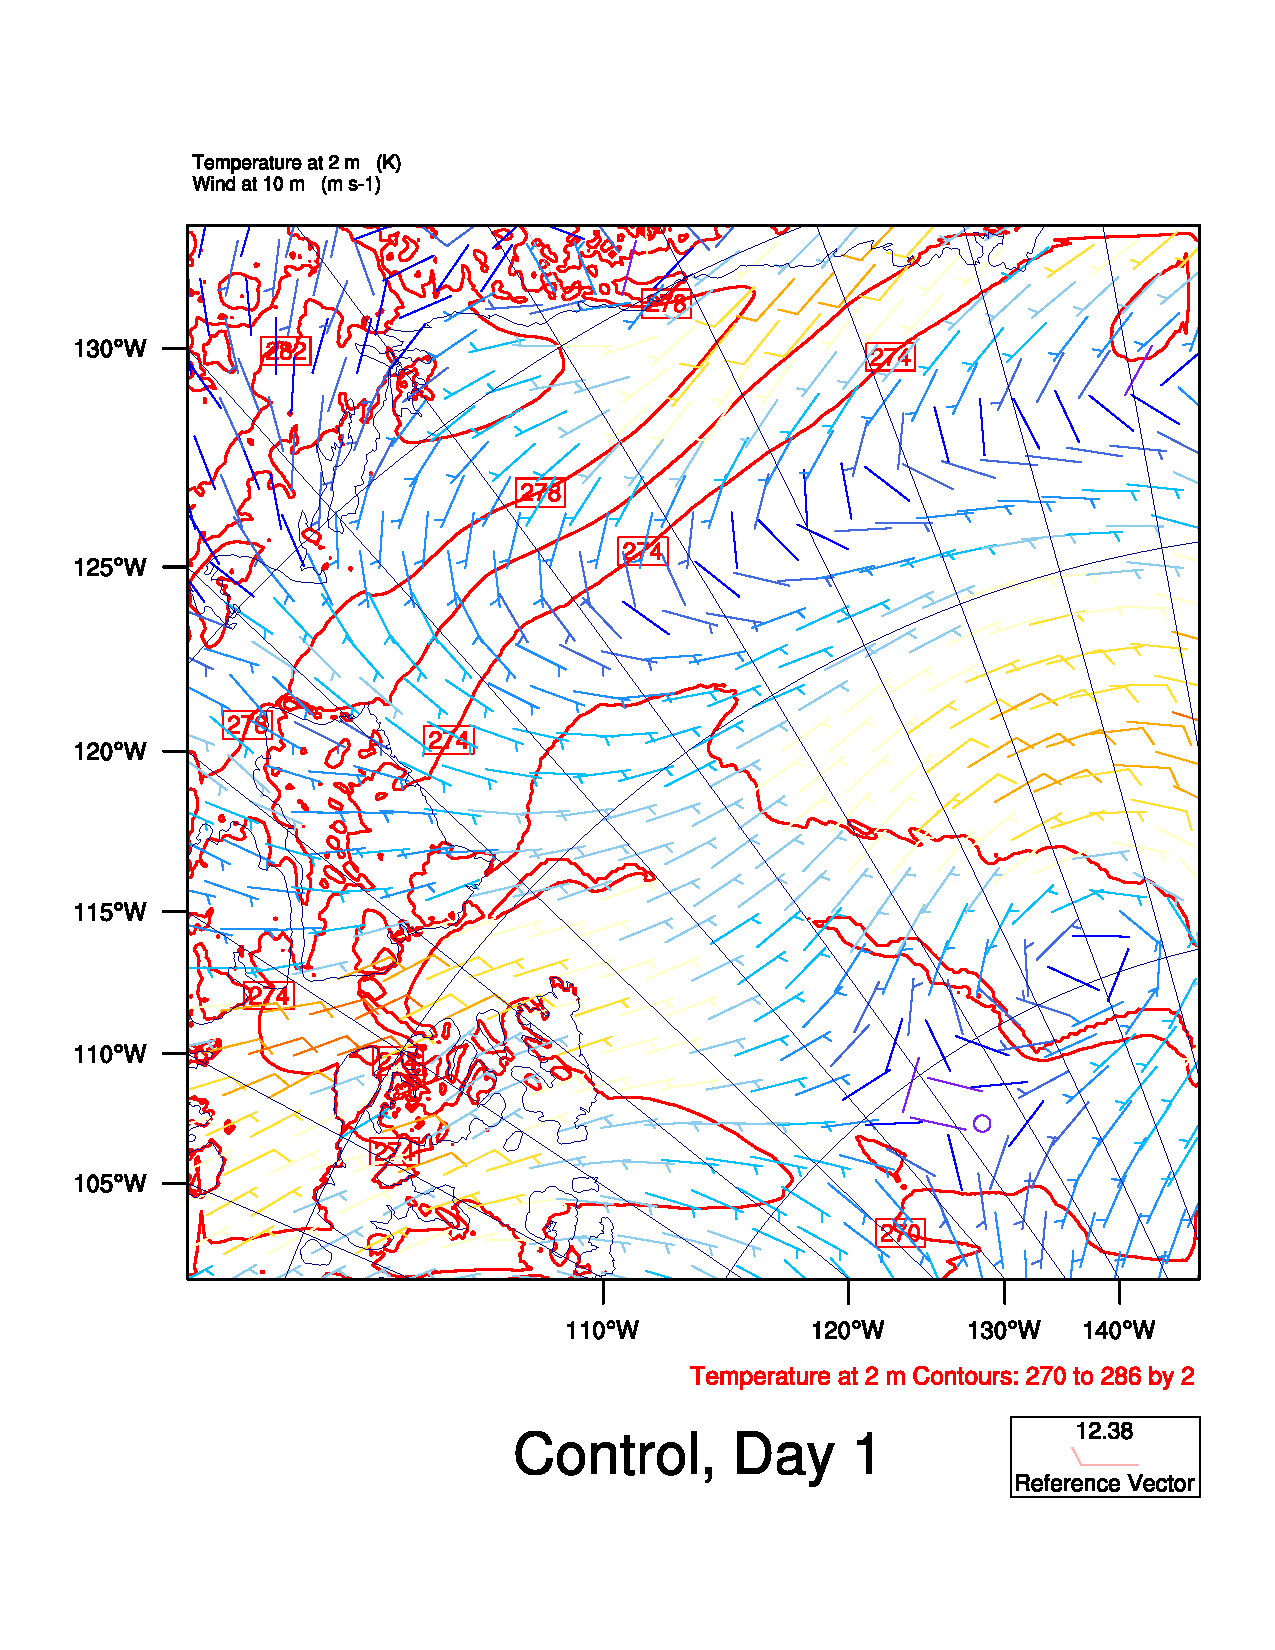
\includegraphics[width=\textwidth]{results/T2UV10_Control_Day1.pdf}
        \caption{Day 1}
        \label{subfig:weather_cont_day1}
    \end{subfigure}
    \begin{subfigure}{0.48\textwidth}
        \centering
        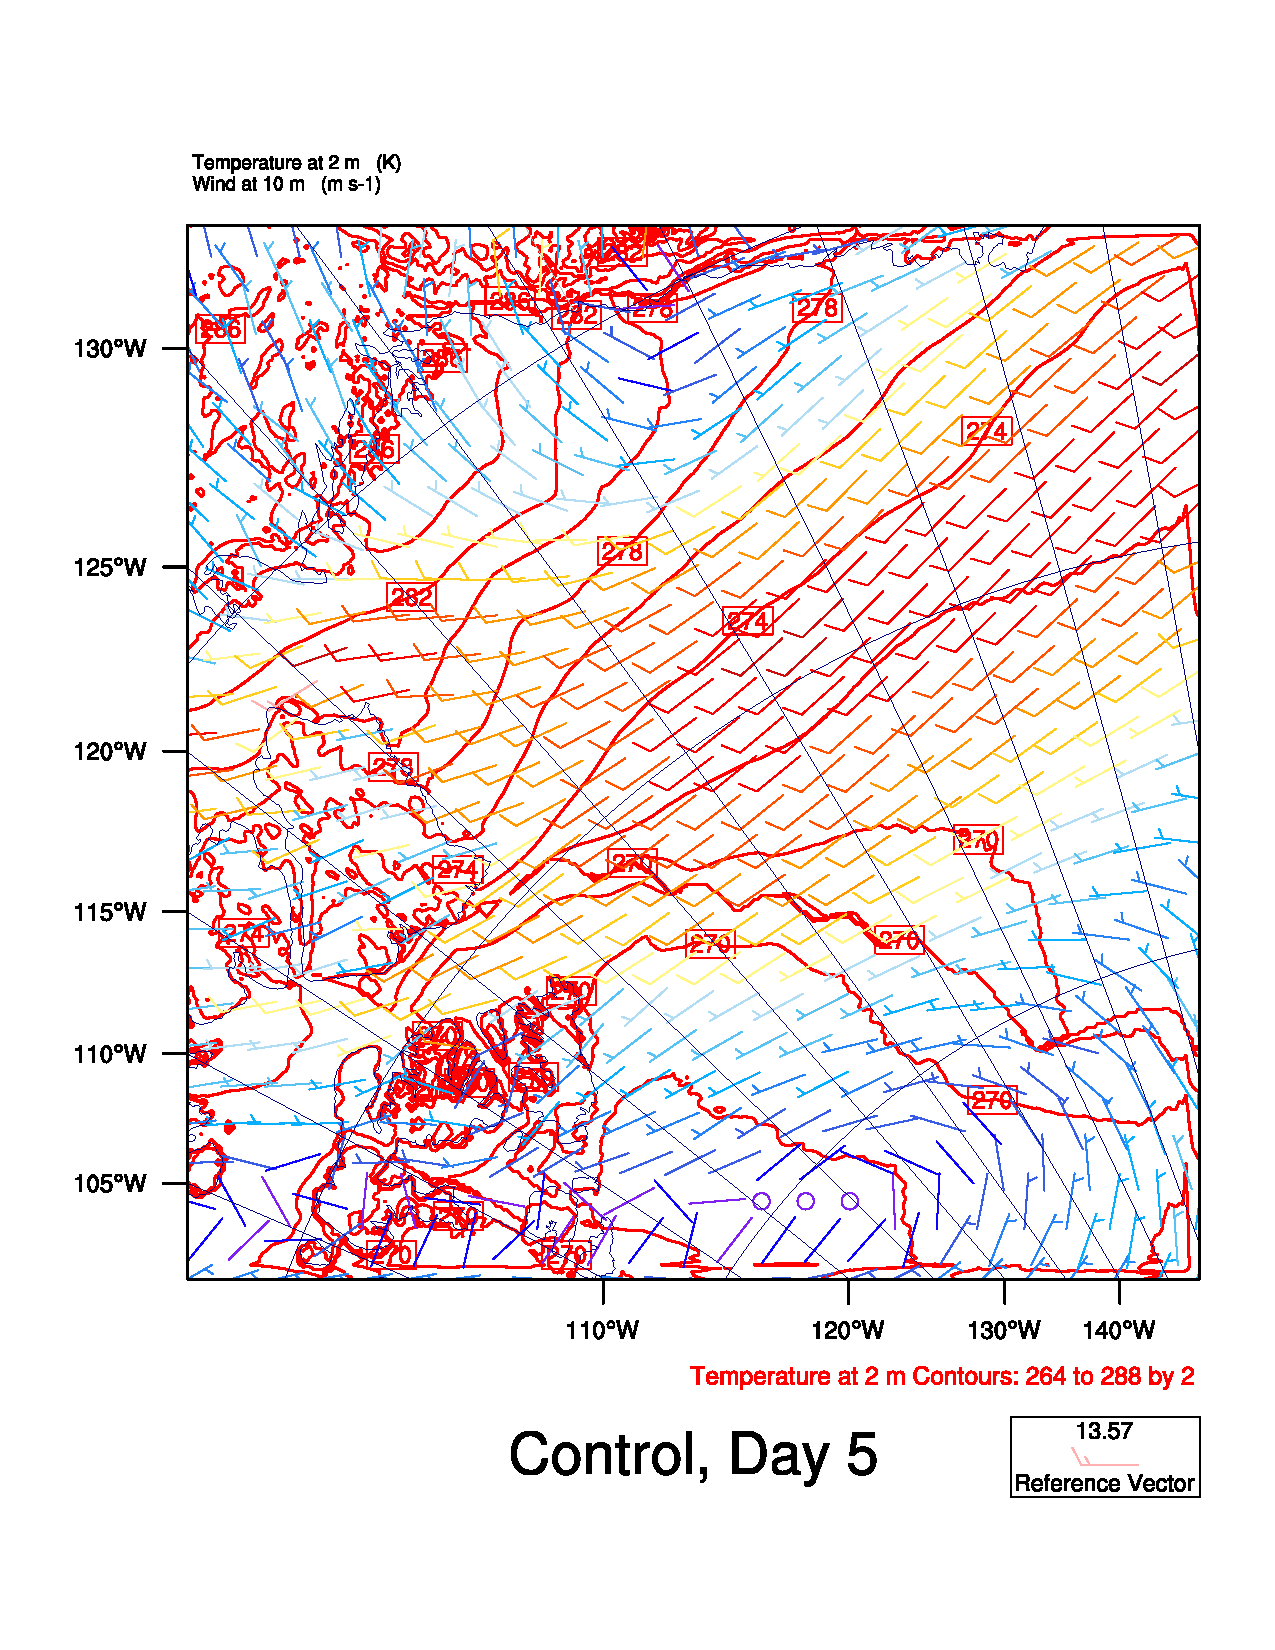
\includegraphics[width=\textwidth]{results/T2UV10_Control_Day5.pdf}
        \caption{Day 5}
        \label{subfig:weather_cont_day5}
    \end{subfigure}
    \caption{The temperature and wind pattern for days 1 and 5, from the control run. The temperature at 2~m height is represented by red contour lines and the wind speed and direction at 10~m height is shown by wind barbs and their color, where red is higher wind speed and blue is lower. The shortest tails on the wind barbs indicate 2.5~m/s each, the longer tails indicate 5~m/s and the longest indicate 10~m/s.}
    \label{fig:weather}
\end{figure}

By day 5 the wind direction has changed to south-easterly, see figure~\ref{subfig:weather_cont_day5}, and the clouds in the cross section, figure~\ref{subfig:cross_LWC_Day5} are low stratus over the sea ice, and there is also some thin cloud formation at the mountain, probably formed by weaker orographic lifting. There is no IWC in the section for day 5 (not shown).

\begin{figure}[h]
    \centering
    \begin{subfigure}{0.48\textwidth}
        \centering
        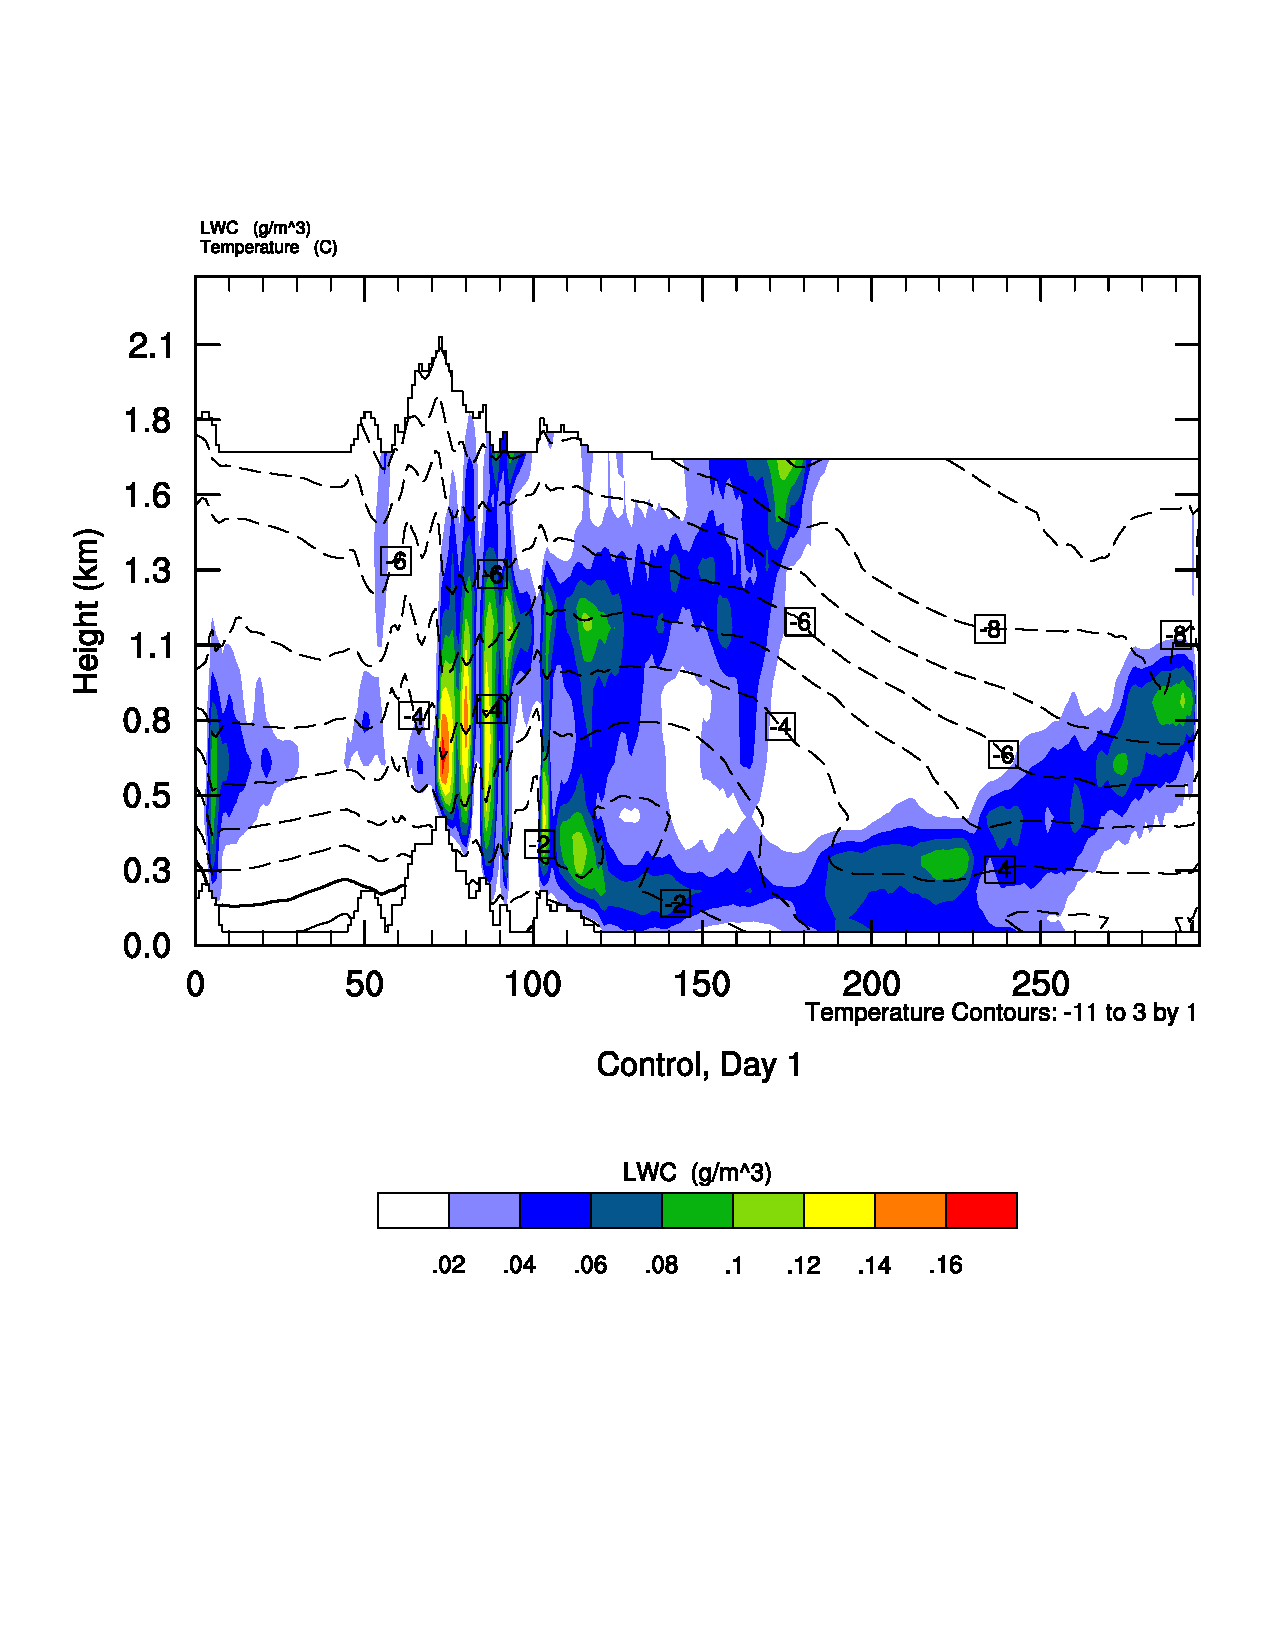
\includegraphics[width=\textwidth]{results/crossSec_LWC_Control_Day1.pdf}
        \caption{LWC, control run, day 1.}
        \label{subfig:cross_LWC_day1}
    \end{subfigure}
    \begin{subfigure}{0.48\textwidth}
        \centering
        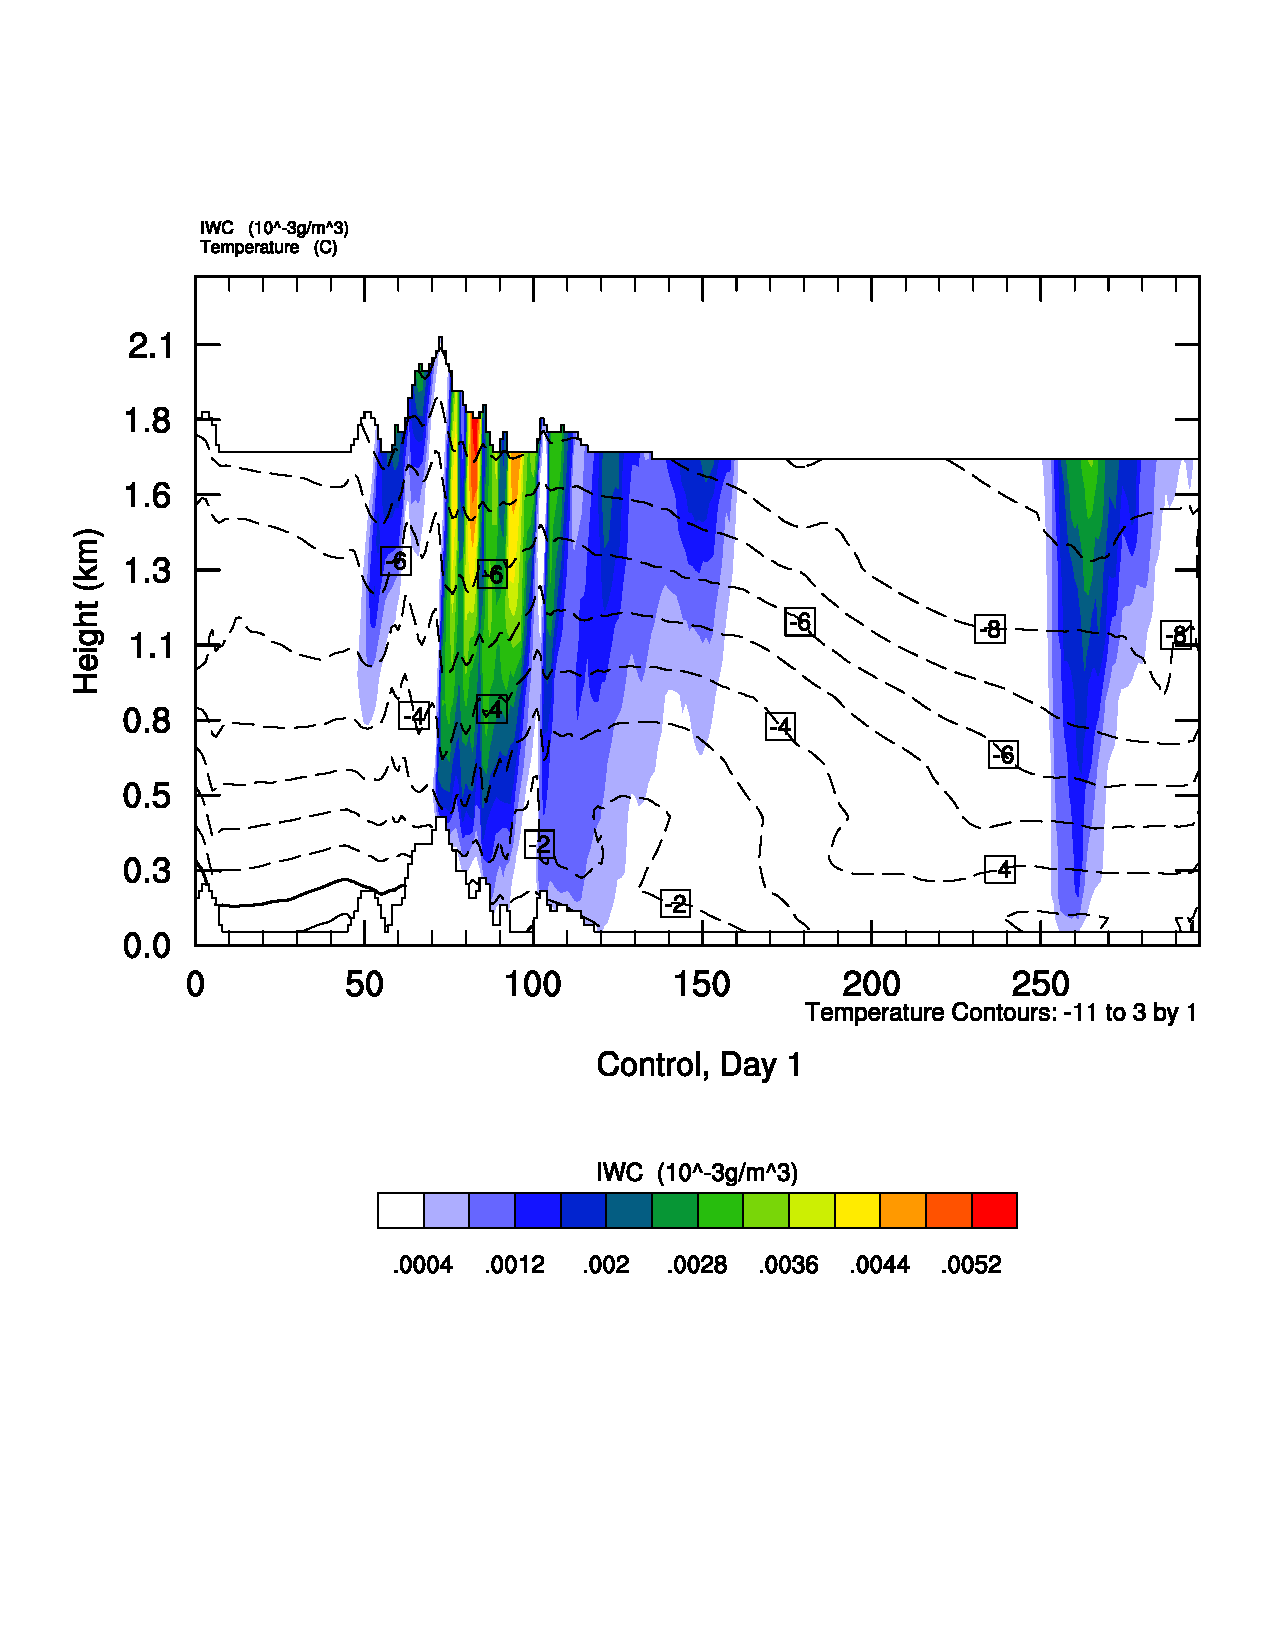
\includegraphics[width=\textwidth]{results/crossSec_IWC_Control_Day1.pdf}
        \caption{IWC, control run, day1.}
        \label{subfig:cross_IWC_day1}
    \end{subfigure}
    
    \begin{subfigure}{0.48\textwidth}
        \centering
        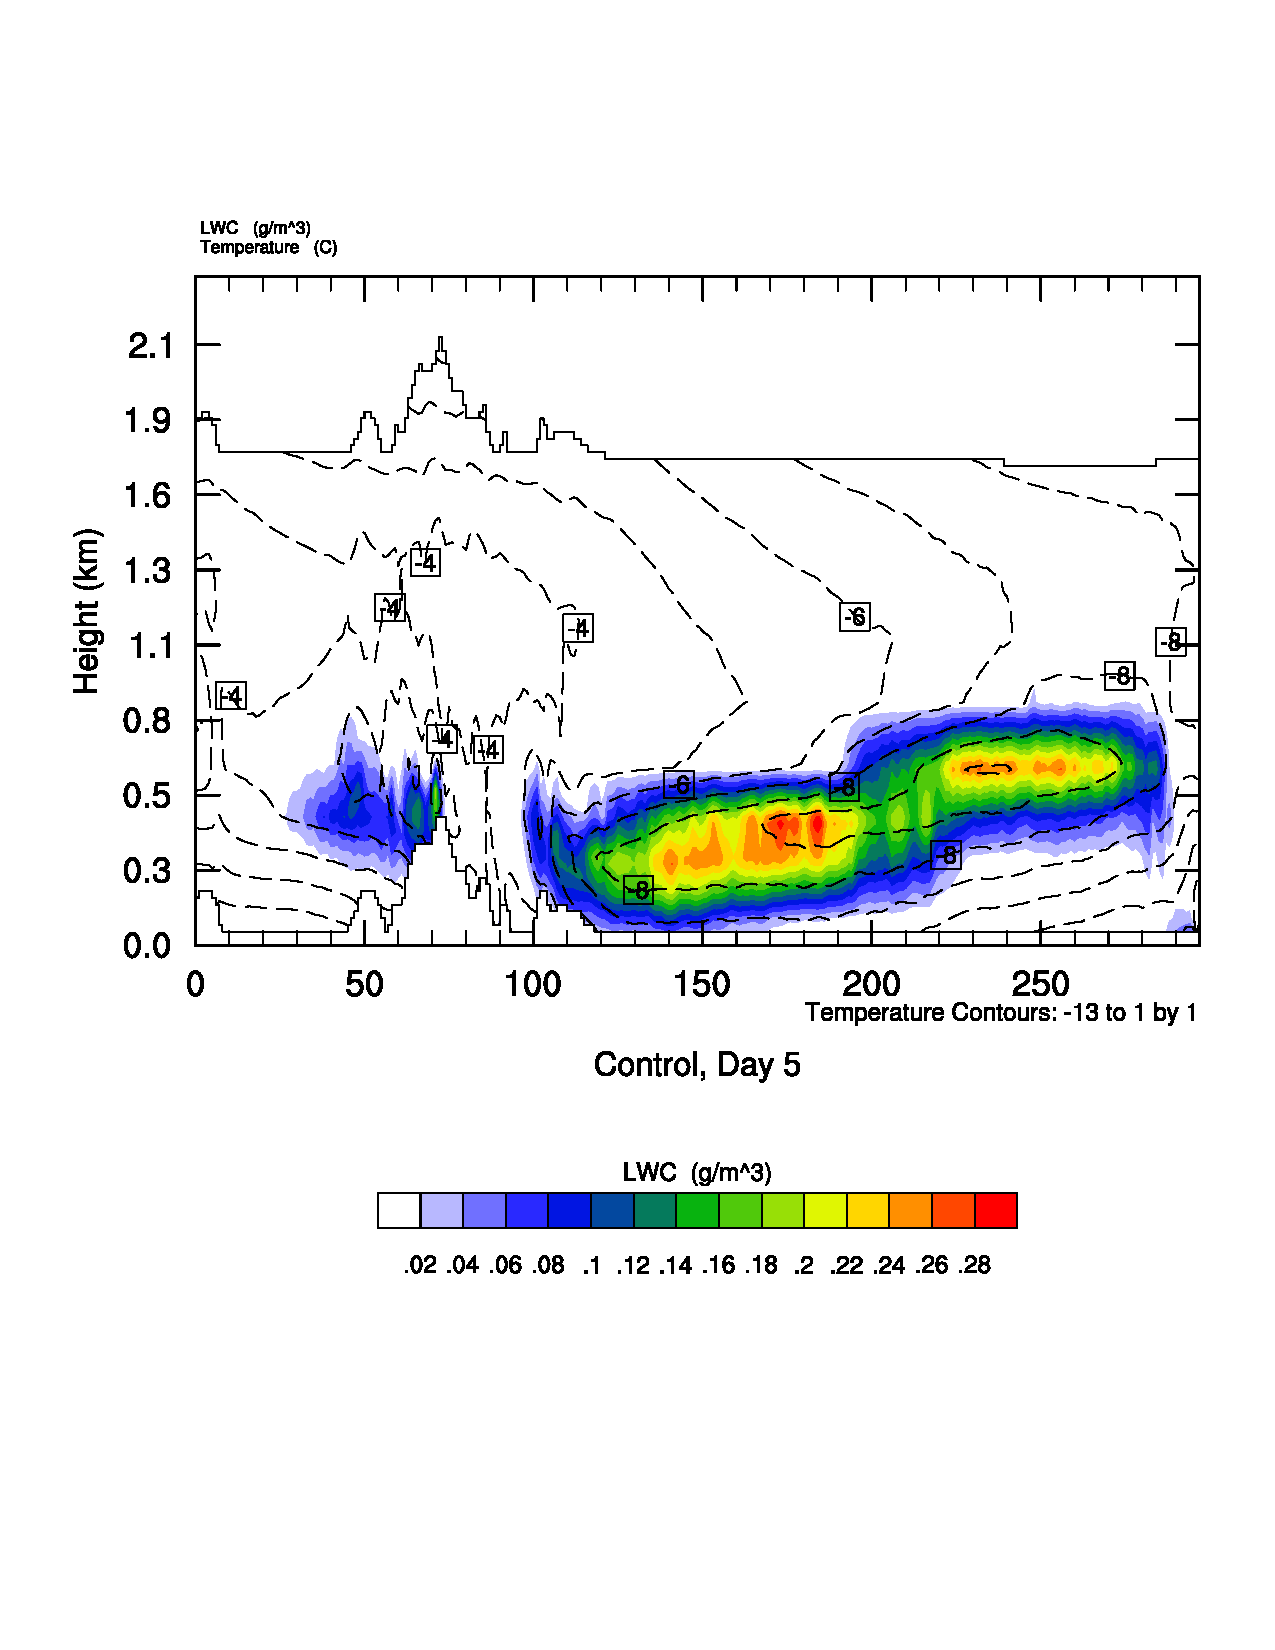
\includegraphics[width=\textwidth]{results/crossSec_LWC_Control_Day5.pdf}
        \caption{LWC, control run, day 5.}
        \label{subfig:cross_LWC_Day5}
    \end{subfigure}
    \begin{subfigure}{0.48\textwidth}
        \centering
        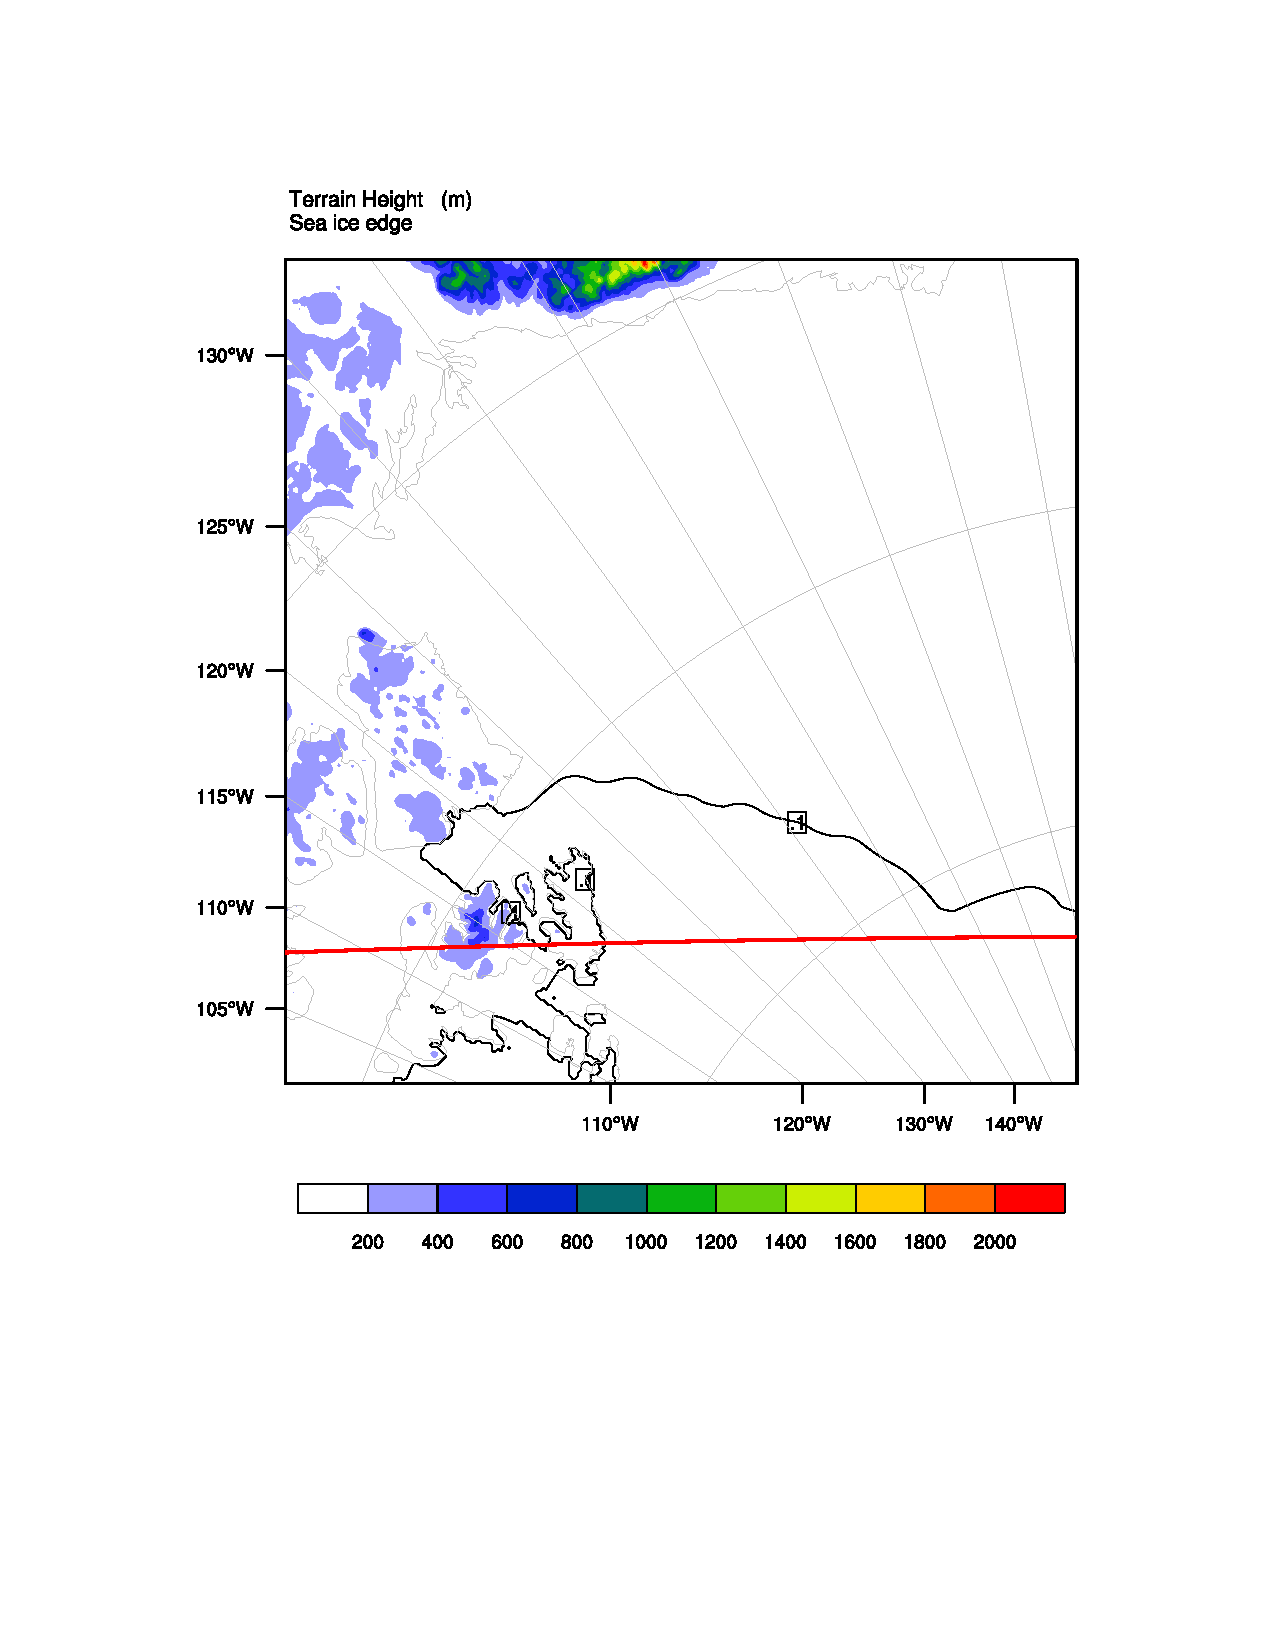
\includegraphics[width=\textwidth]{results/crossSec_line.pdf}
        \caption{Line over which the vertcal cross sections are made.}
        \label{subfig:cross_line}
    \end{subfigure}
    \caption{Vertical cross sections of averaged liquid ($\text{g/m}^3$) and ice  ($\text{mg/m}^3$) water content, and temperature ($\degree\text{C}$), from the control run, for days 1 and 5. LWC and IWC for day 1 are shown in figures~\ref{subfig:cross_LWC_day1} and~\ref{subfig:cross_IWC_day1} respectively. Figure~\ref{subfig:cross_LWC_Day5} shows the LWC for day 5. The IWC on day 5 was 0 in the section and is not shown. Figure~\ref{subfig:cross_line} shows a map of the area with the ice edge as a black contour line. The terrain height is represented by filled contours and the red line over the sea ice is the line over which the cross sections are made.}
    \label{fig:weather}
\end{figure}

The LWP for day 1 and 5 is shown in figure (@subfig) and (@subfig) with the CDNC (@subfig) and (@subfig) and $r_e$ (@subfig) and (@subfig). One can clearly see that where the LWP is high, so is the CDNC, which is expected based on equation~\ref{eqn:LWC}. The pattern in $r_e$ is @different due to...@

The fluxes of both SW and LW radiation at both the surface and at the top of the atmosphere (TOA) may be partly explained by the clouds, through looking at the LWP. Figure (@radiation) shows the downward SW at the surface (@subfig) and upward at TOA (@subfig) for day 1 and @more radiation and why it looks that way.

The heat fluxes upward at the surface, latent heat (LH) and sensible heat (SH), are also of interest when studying clouds in the Arctic. The fluxes are shown in figure (@figure) for day 1 (LH (@subfig), SH (@subfig)) and day 5 (LH (@subfig), SH (@subfig)). Notice that the LH and SH is lower over the sea ice for both days 1 and 5. This because the sea ice is colder than the ocean, and works as a lid over that part of the ocean, not letting all the heat out.

%--------- Cloud droplet and ice number concentrations
\begin{figure}[h]
\centering
\includegraphics[width=0.5\textwidth]{results/cdnc_cont_day1.png}
\caption{Cloud droplet number concentration, averaged over the lower 11 layers and the 1st day.}
\label{fig:cdnc_cont_Day1}
\end{figure}

\begin{figure}[h]
\centering
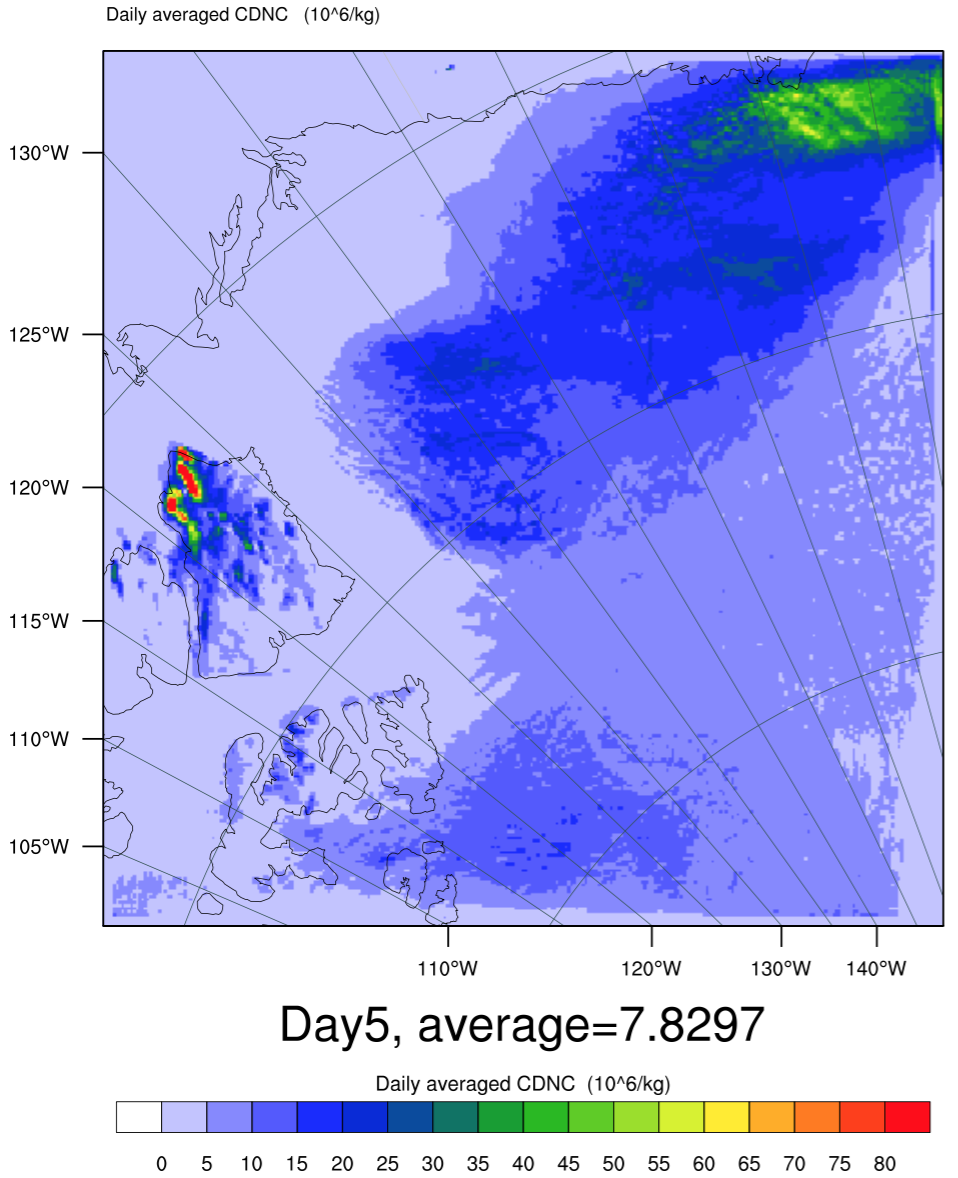
\includegraphics[width=0.5\textwidth]{results/cdnc_cont_day5.png}
\caption{Cloud droplet number concentration, averaged over the lower 11 layers and the 5th day.}
\label{fig:cdnc_cont_Day5}
\end{figure}

\begin{figure}[h]
\centering
\includegraphics[width=0.5\textwidth]{results/cinc_cont_day1.png}
\caption{Cloud ice number concentration, plotted over the area, averaged over the lower 11 layers on the 1st day.}
\label{fig:cinc_cont_Day1}
\end{figure}

\begin{figure}[h]
\centering
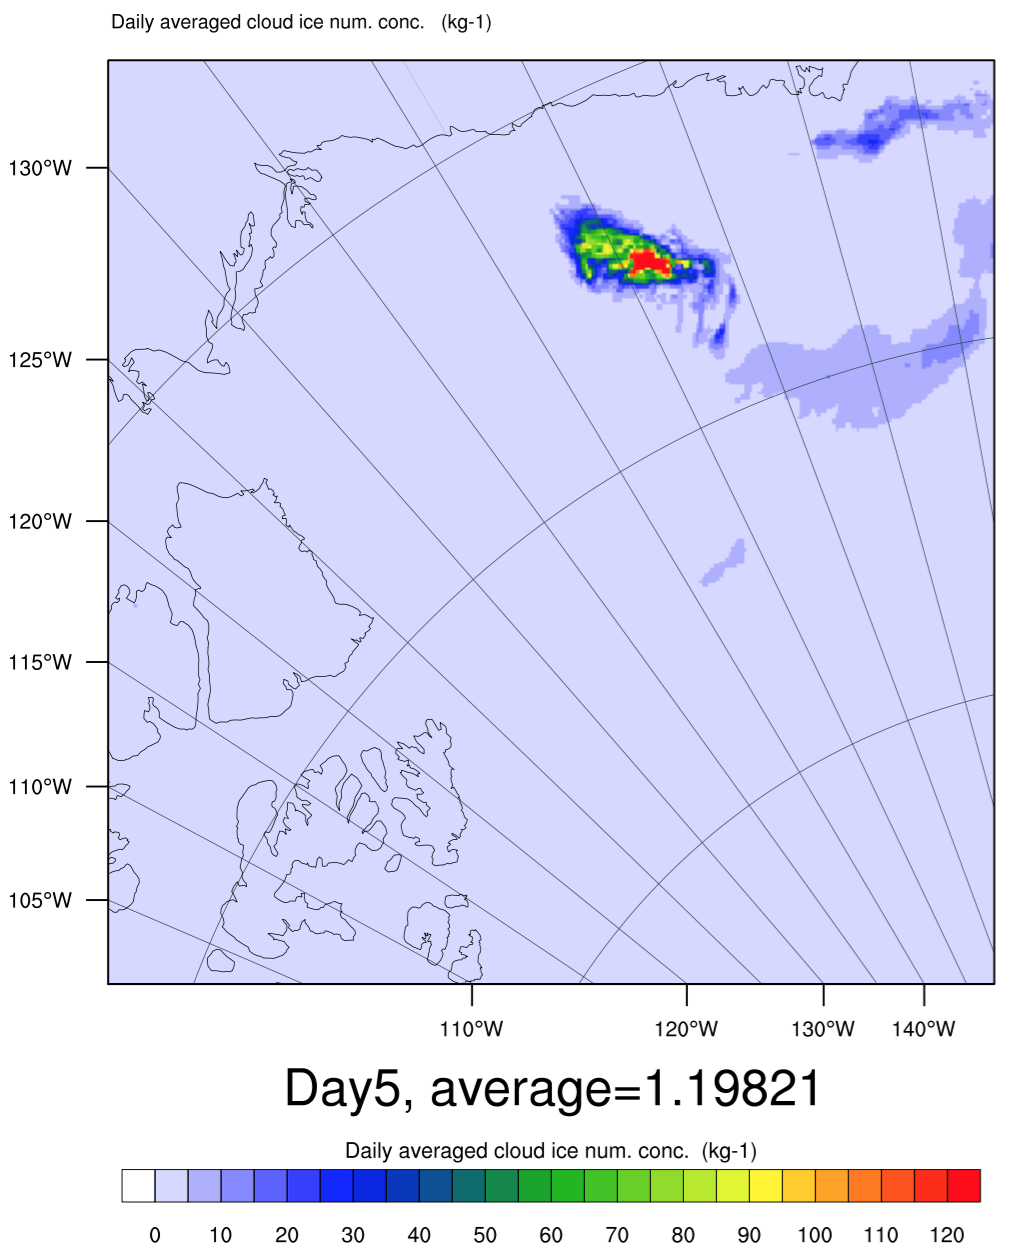
\includegraphics[width=0.5\textwidth]{results/cinc_cont_day5.png}
\caption{Cloud ice number concentration, plotted over the area, averaged over the lower 11 layers on the 5th day.}
\label{fig:cinc_cont_Day5}
\end{figure}

%---------- LWP control run, days 1 and 5

\begin{figure}
    \centering
    \begin{subfigure}{0.48\textwidth}
        \centering
        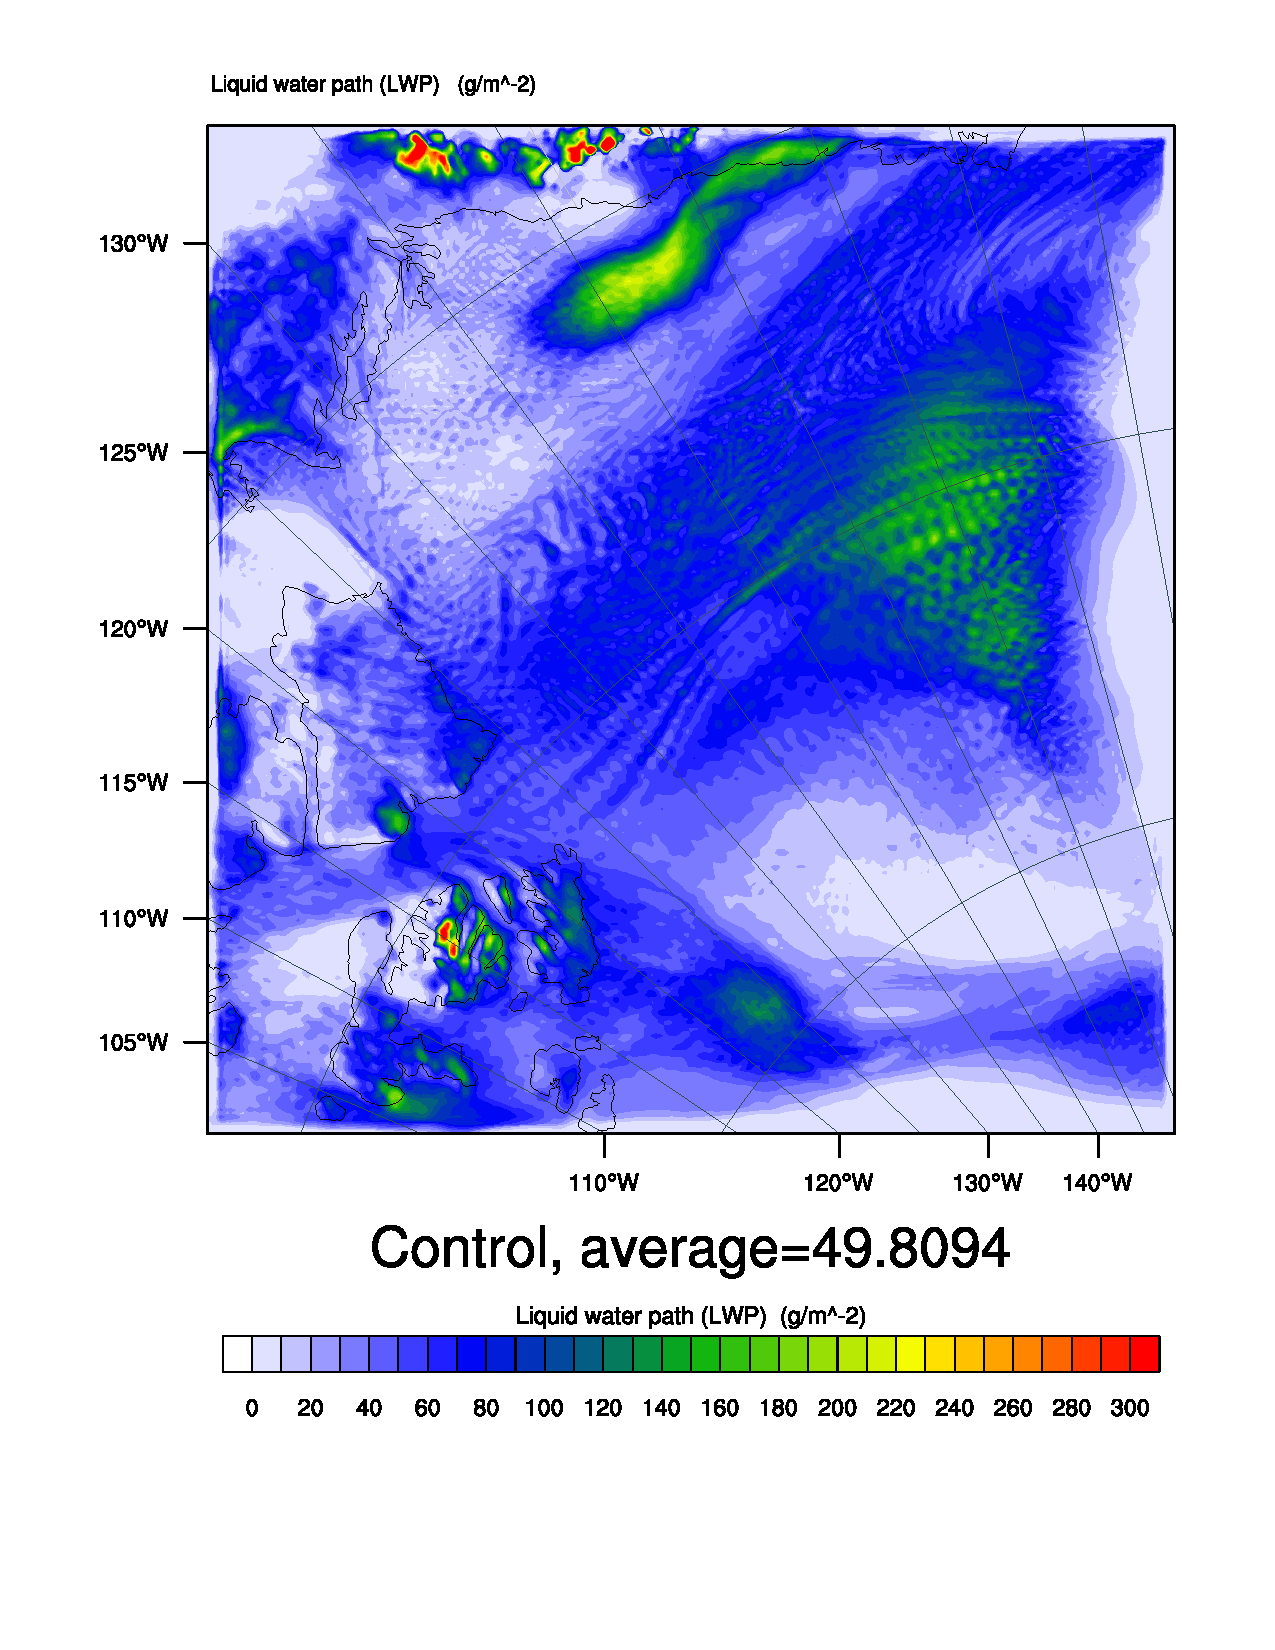
\includegraphics[width=\textwidth]{results/LWP_Day1.pdf}
        \caption{Day 1}
        \label{subfig:LWPr1Day1}
    \end{subfigure}
    \begin{subfigure}{0.48\textwidth}
        \centering
        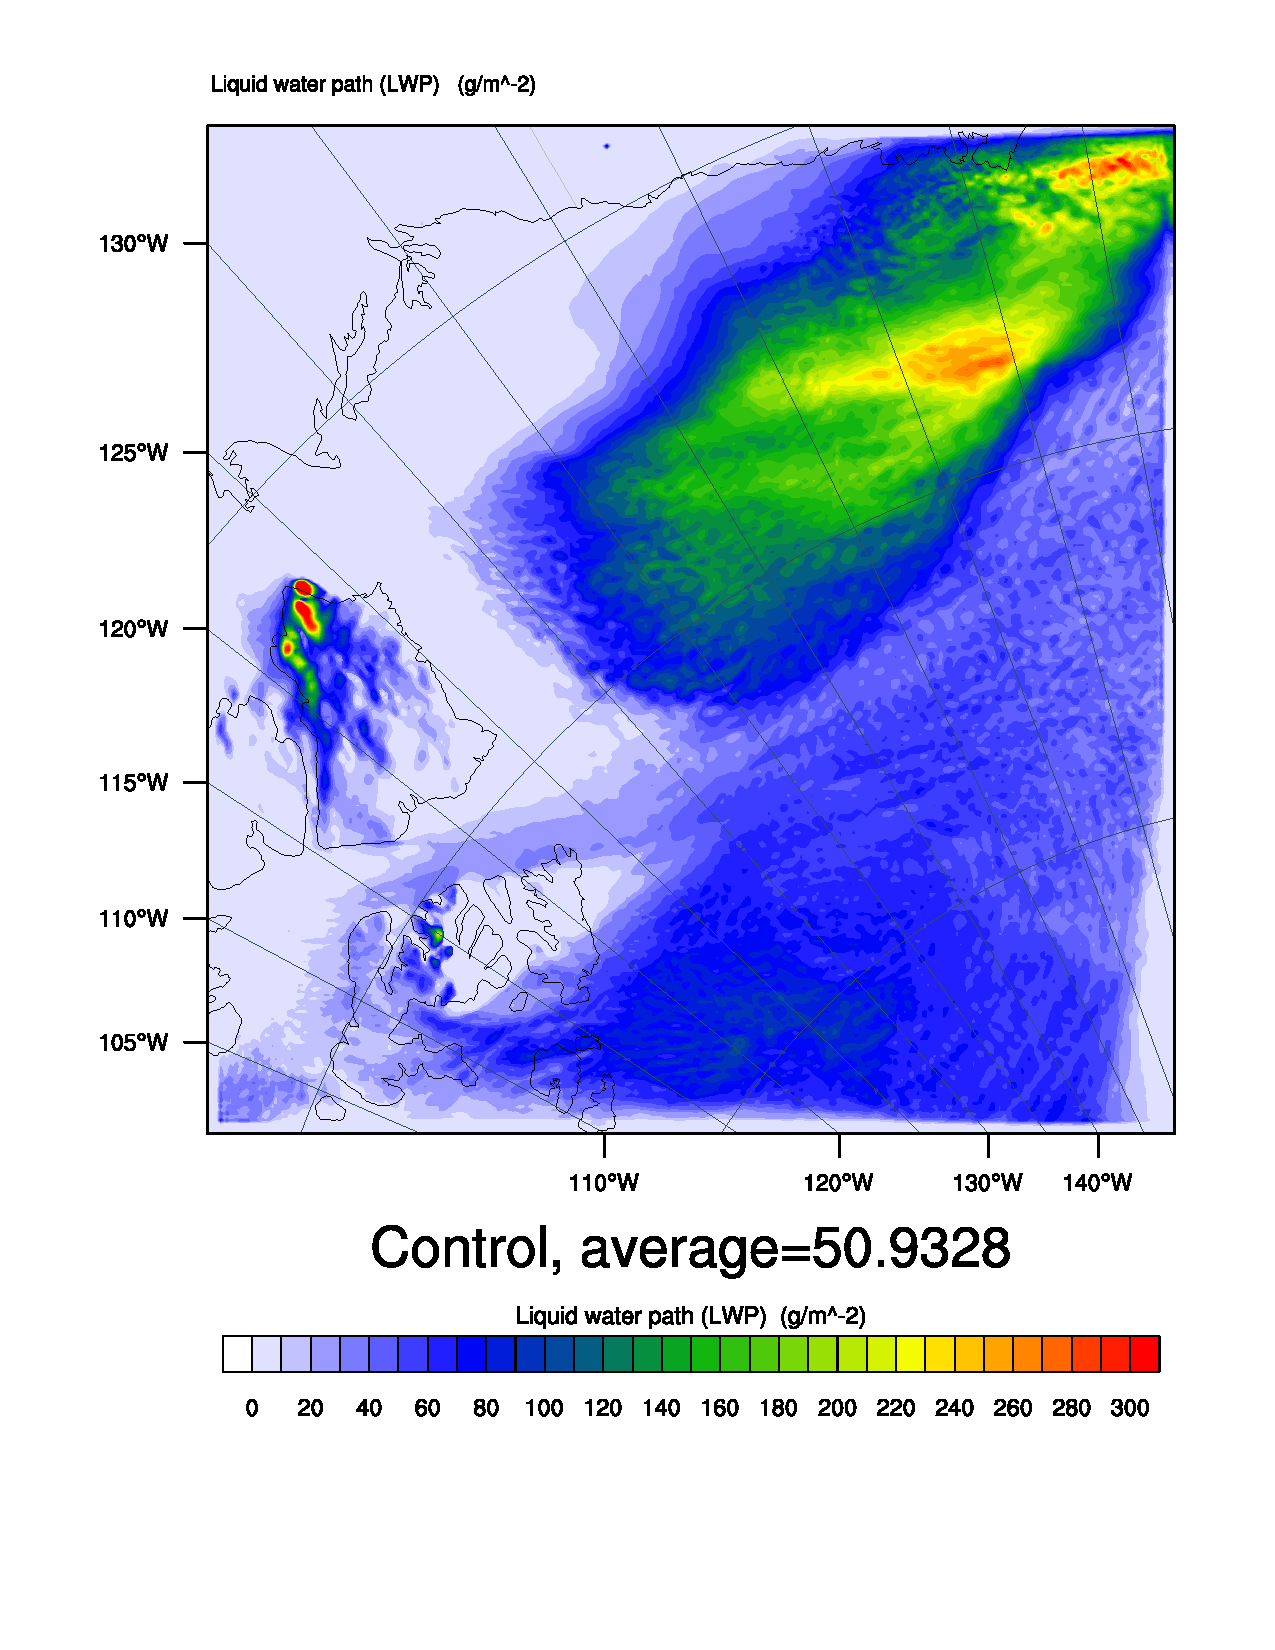
\includegraphics[width=\textwidth]{results/LWP_Day5.pdf}
        \caption{Day 5}
        \label{subfig:LWPr1Day5}
    \end{subfigure}
    \caption{The average liquid water path (LWP) for days 1 and 5, including the average value for the field.}
    \label{fig:LWP}
\end{figure}
%----------- Effective radius, days 1 and 5

\begin{figure}[h]
\centering
\includegraphics[width=0.5\textwidth]{results/recloud_cont_day1.png}
\caption{The effective radius of cloud droplets average field for day 2 over the lowermost 11 layers.}
\label{fig:recloud_r1Day1}
\end{figure}

\begin{figure}[h]
\centering
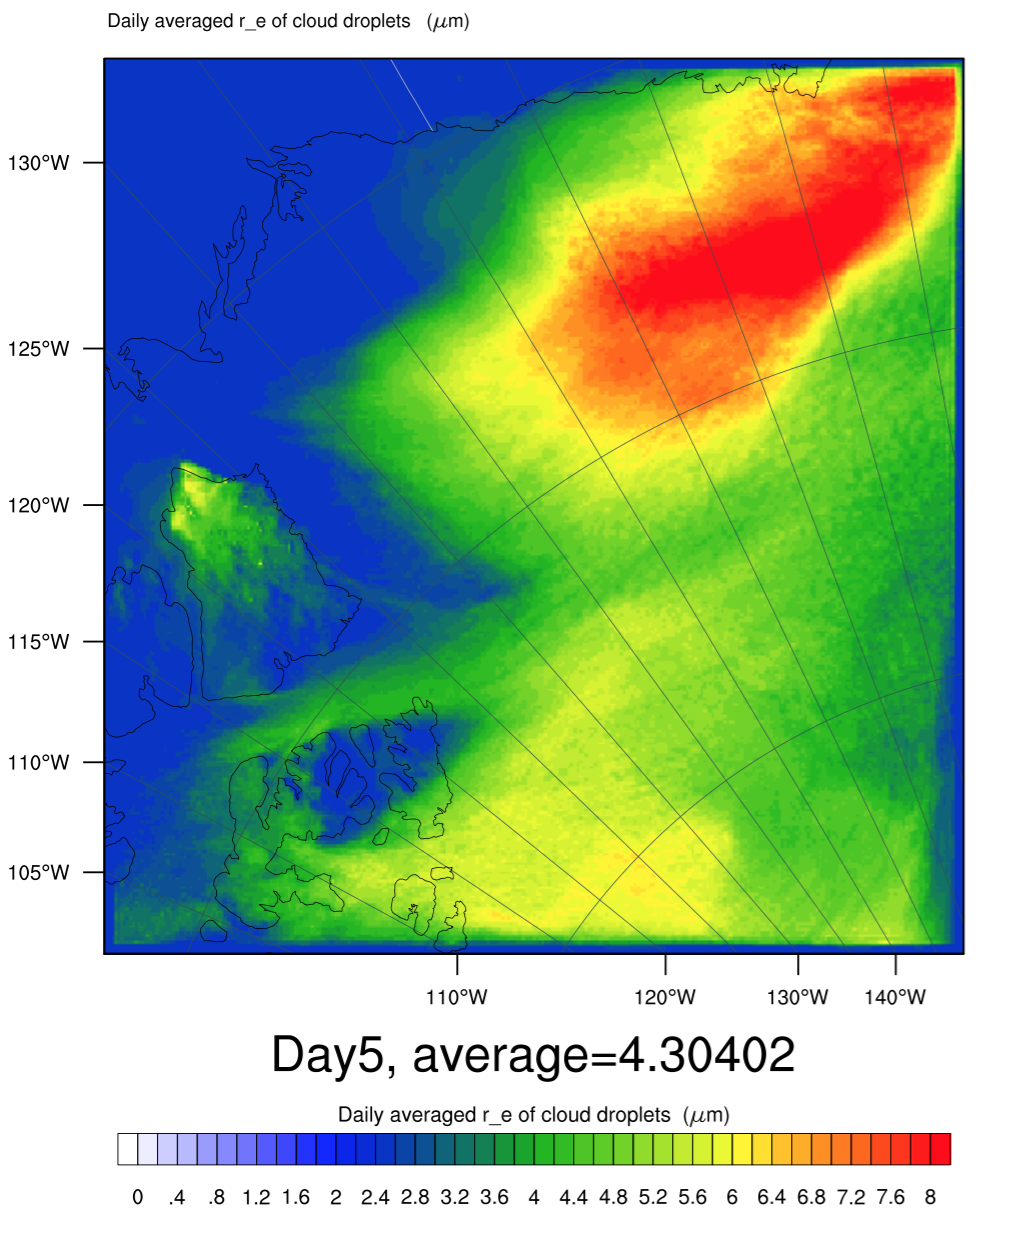
\includegraphics[width=0.5\textwidth]{results/recloud_cont_day5.png}
\caption{The effective radius of cloud droplets average field for day 5 over the lowermost 11 layers.}
\label{fig:recloud_r1Day5}
\end{figure}


---------

%First we want to have something to compare with and to look back to when studying the differences from the control run to the runs with changed sea ice and/or aerosol concentration. I shall include figures for diurnally averaged fields of LWP, $r_e$ of cloud droplet, cloud droplet number concentration (CDNC), both LW and SW up at the TOA and down at the surface. Also the IWP, cloud ice number concentration (CINC), and $r_e$ of snow and ice may be of interest. In addition, the state of the weather situation should be considered when interpreting the results. Therefore maps with wind barbs for the wind at 10~m height and temperature at 2~m are included in this section.

%-----------------------
\section{Removed sea ice}
%-----------------------
\subsection{Day 1}
Lets start with average difference in LWP for NoIce - Control, day 1 (see figure~\ref{fig:relwpcdnc_r2Day1}). There is a slight difference in LWP for the whole field (@$gm^{-2}$, see figure~\ref{fig:relwpcdnc_r2Day1}), but the area of interest in this case is where the sea ice is no longer present. There the increase in LWP is significantly higher, >@$gm^{-2}$ for the most northern part (which is in the bottom right corner). This implies that there is a new cloud forming in that area, that could not form when there was sea ice. The removal of the sea ice has allowed for increased evaporation and an increase in latent heat (LH) flux which can be seen from figure~\ref{fig:lhdiff_r2Day1}, where the area that sea ice was removed from is obvious. The northernmost part of the study area also has an increase in the cloud droplet number concentration (CDNC), figure~\ref{fig:relwpcdnc_r2Day1}, with about the same shape and size as the LWP, which fits well with equation~\ref{eqn:lwc_prop_cdnc}, which we know from the theory presented in chapter~\ref{chap:theory}. 

\begin{figure}[h!]
\centering
\includegraphics[width=\textwidth]{results/cdnclwpre_r2Day1.png}
\caption{The averaged difference in $r_e$ of cloud droplets, LWP and CDNC (from left to right) for the run with no ice, over the lowermost 11 layers for day 2. (preliminary figure)}
\label{fig:relwpcdnc_r2Day1}
\end{figure}

The amount of liquid water is proportional to the number concentration, and the LWP is the integral over the LWC, where we recall that N is the CDNC. The average increase in the CDNC would be approximately 5 droplets per cubic centimeter. The figure shows the numbers with units $10^6/kg$, which can be approximated to the more common units for CDNC, per cubic centimeter ($cm^{-3}$). If we assume that we are close enough to the surface to assume a pressure $p=1000hPa$, and thereby the density to be $\rho_a = 1kg/m^3=1kg/10^6cm^3$, then we could write $CDNC : 10^6/kg = cm^{-3}$. Since this is the average over 11 layers, to a height of about 1600~m, the cloud could be in just a few of those layers, and have a CDNC of approximately 25 $cm^{-3}$ if it stretches over two layers for example. The increase in effective radius in the same area also indicates the formation of a new cloud,figure~\ref{fig:relwpcdnc_r2Day1}, that could not form in the control run (see figure~\ref{fig:recloud_r1Day1}), whereas now that it has formed, the droplets actually have a radius. The small "blob" at 140$^o$W and about 81$^o$N has decreased $r_e$, most likely because the cloud already was saturated in that area, which can be seen from the LWP from the control run, in figure~\ref{fig:LWPr1Day1}. The possible increase in aerosols from the ocean that would then lead to an increase in CCNs would make the water in that cloud spread over more CCNs, and by that leave the droplets with a smaller $r_e$.

\begin{figure}
\centering
\includegraphics[width=0.6\textwidth]{results/diff_NoIce_lh_Day2.png}
\caption{The average difference in LH flux up from the surface at day 2 .}
\label{fig:lhdiff_r2Day2}
\end{figure}

The kind of U-shape that we can see in the figure for difference in $r_e$, figure~\ref{fig:relwpcdnc_r2Day2}, is also clear in the difference in downward radiation at the ground surface, for both SW and LW. The SW radiation flux at ground surface has been reduced, which is due to the increase in LWP. This can be explained by equations~\ref{eqn:cloudalbedo} and~\ref{eqn:cloudtau}, where it is clear from equation~\ref{eqn:cloudtau} that the cloud optical depth, $\tau$, increases with LWP, and from equation~\ref{eqn:cloudalbedo} it is clear that an increase in $\tau$ would also increase the cloud albedo.

The downward LW radiation flux at the surface has been increased due to the increase in LWP, which means that there is more water in the clouds and they emit more LW to the ground. It was shown in Chapter~\ref{chap:theory} that an increase in LWP increases increases the emissivity of the cloud, shown in equation~\ref{eqn:epsilon_lw}. The LW at the top of the atmosphere (TOA) does not experience such an increase, in fact it experiences a slight decrease. That it doesn't experience the same increase is explained by the Stefan-Boltzmann's law presented in chapter~\ref{chap:theory}, where the flux density emitted by a body, in this case a cloud, is dependent on the temperature. % equation for cloud LW emissivity(@refer, but find it first!), which is dependent of temperature.
\textit{ We see from the vertical cross section showing temperature contours (@refer and make), that the temperature is higher at the surface than in the clouds, therefore the clouds have a lower emittance of LW. (this figure will come in the next draft, but is currently not averaged)}
%The removal of sea ice has a larger effect on lower clouds than on higher clouds, since the increase in evaporation from the surface doesn't reach high up in the troposphere, especially not in the Arctic, due to the static stability of the lower atmosphere in the Arctic(@cite someone?). Also the LWP showed in this study is only for the lowermost 11 layers and can only explain what happens in those layers, it can not be used as a final explanation for radiation changes that are only at the bottom and top of the modeled atmosphere.

\begin{figure}
\centering
\includegraphics[width=0.6\textwidth]{results/diff_NoIce_swup_Day2.png}
\caption{The average difference in SW flux up at TOA at day 2 .}
\label{fig:swupdiff_r2Day2}
\end{figure}
%Include figure with vertical temperature changes? or just show vertical temperature for all runs in one plot with subplots?
Of course, the removal of sea ice would reduce the reflected SW radiation flux at the TOA, see figure~\ref{fig:swupdiff_r2Day2}. The albedo of sea ice varies between 0.5 and 0.9 depending on snow cover and the age of the ice and is typically 0.5-0.7 for bare ice, whereas a typical ocean albedo is 0.06. Thus the change in SW at TOA is mainly negative over the area of ocean where there was sea ice in the control run. The two blobs of increased SW at TOA, see figure~\ref{fig:swupdiff_r2Day2}, can be recognized as the tips of the pillars in the U-shape I referred to for $r_e$ earlier (in figure~\ref{fig:relwpcdnc_r2Day2}) which also represent an increase in LWP and reduction in SW at surface and increase of LW at surface. This is therefore most likely due to the enhanced albedo caused by new clouds at those locations, since these figures don't show in-cloud changes, simply the difference between two fields.

\begin{figure}
\centering
\includegraphics[width=0.6\textwidth]{results/diff_NoIce_hfx_Day2.png}
\caption{The average difference in SH flux up from the surface at day 2 .}
\label{fig:shdiff_r2Day2}
\end{figure}

The heat fluxes are almost unchanged for most of the study area by the removal of sea ice, except for the area where the sea ice has been removed (see figures~\ref{fig:lhdiff_r2Day2} and~\ref{fig:shdiff_r2Day2}). Especially for the northernmost part of the study area and "sea ice removed area" the fluxes are a lot higher than in the control run. This is not surprising, since one would expect the ocean surface to hold a higher temperature than the sea ice. Also a lot more heat would be released due to evaporation than in the case when sea ice is present.

\subsection{Day 5}
I still can't explain what is going on i figure~\ref{fig:relwpcdnc_r2Day5}. I have tried to look into differences in rain, and snow, and graupel and ice content, but I can't seem to figure it out...
\begin{figure}[h!]
\centering
\includegraphics[width=\textwidth]{results/cdnclwpre_r2Day5.png}
\caption{The average differences in $r_e$, LWP and CDNC from left to right, for day 5. (preliminary figure)}
\label{fig:relwpcdnc_r2Day5}
\end{figure}
%Why the crap does the effective radius, LWP and CDNC go down significantly and simultaneously for the removal of sea ice at day 5?? What is up with this system? Could it be rain? From the figure I made it doesn't look like it is due to rain, 'cause it actually looks like rain is also reduced in this case, which is STRANGE!... what??? And the heat flux differences also look crazy, very clear increase right next to an equally clear decrease, the switch happens at the sea ice edge. That makes sense :) but the rest doesn't!!
%Jon Egill suggested that I check ice and snow too, see if that can explain the difference!

%-------------------------------------
\section{Increased aerosol concentration}
%-------------------------------------
\subsection{Day2}
The increase in available CCNs leads to obvious increases in CDNC and LWP, and the expected reduction in $r_e$, see figure~\ref{fig:cdnclwpre_Aero10}.% If we look back to equation~\ref{eqn:cloudtau}, we see that (@the one that combines LWP, effective radius and cloud optical depth).
\begin{figure}[h!]
\centering
\includegraphics[width=\textwidth]{results/diff_cdnclwpre_Aero10_Day2.png}
\caption{The average differences in $r_e$, LWP and CDNC from left to right, for day 2. (preliminary figure)}
\label{fig:cdnclwpre_Aero10}
\end{figure}

 As for the NoIce run, the increase in LWP, in this case a lot higher, leads to an increase in clouds and their reflectance (albedo), therefore the SW at TOA is higher, here the signal is not disrupted by any changes made to the sea ice, so the increase is obvious, and is shown in figure~\ref{fig:swup_down_r3Day2}. Thus the SW at the surface is significantly lower than in the control run. This represents a cooling of (@calculate the flux changes into temperature changes?). The average LW radiation flux at the surface is higher due to the increase in LWP and thereby increased emittance by the clouds.% thicker and denser(is this true) clouds.
\begin{figure}
\centering
\includegraphics[width=\textwidth]{results/diff_swupdown_Aero10_Day2.png}
\caption{The average difference in SW down at the surface, and up at TOA, from left to right, for day 2. (preliminary figure)}
\label{fig:swup_down_r3Day2}
\end{figure}
The effect on the heat fluxes by increasing the aerosol number concentration is not clear, and probably insignificant (not shown).

\subsection{Day 5}
The LW cloud emissivity is sensitive to an increase in water amount as long as the LWP is less than $\approx$ 40-45 g/m$^2$. It is clear in day 5 from the control run that the LWP was around 60-100 g/m$^2$ in the middle lower area of figure~\ref{fig:LWPr1Day5}.%@ (around these lat and lon?@).
This is also seen in that there is no significant change in LW downward at the surface or upward at the TOA, see figure~\ref{fig:lwup_down_r3Day5}.

\begin{figure}[h!]
\centering
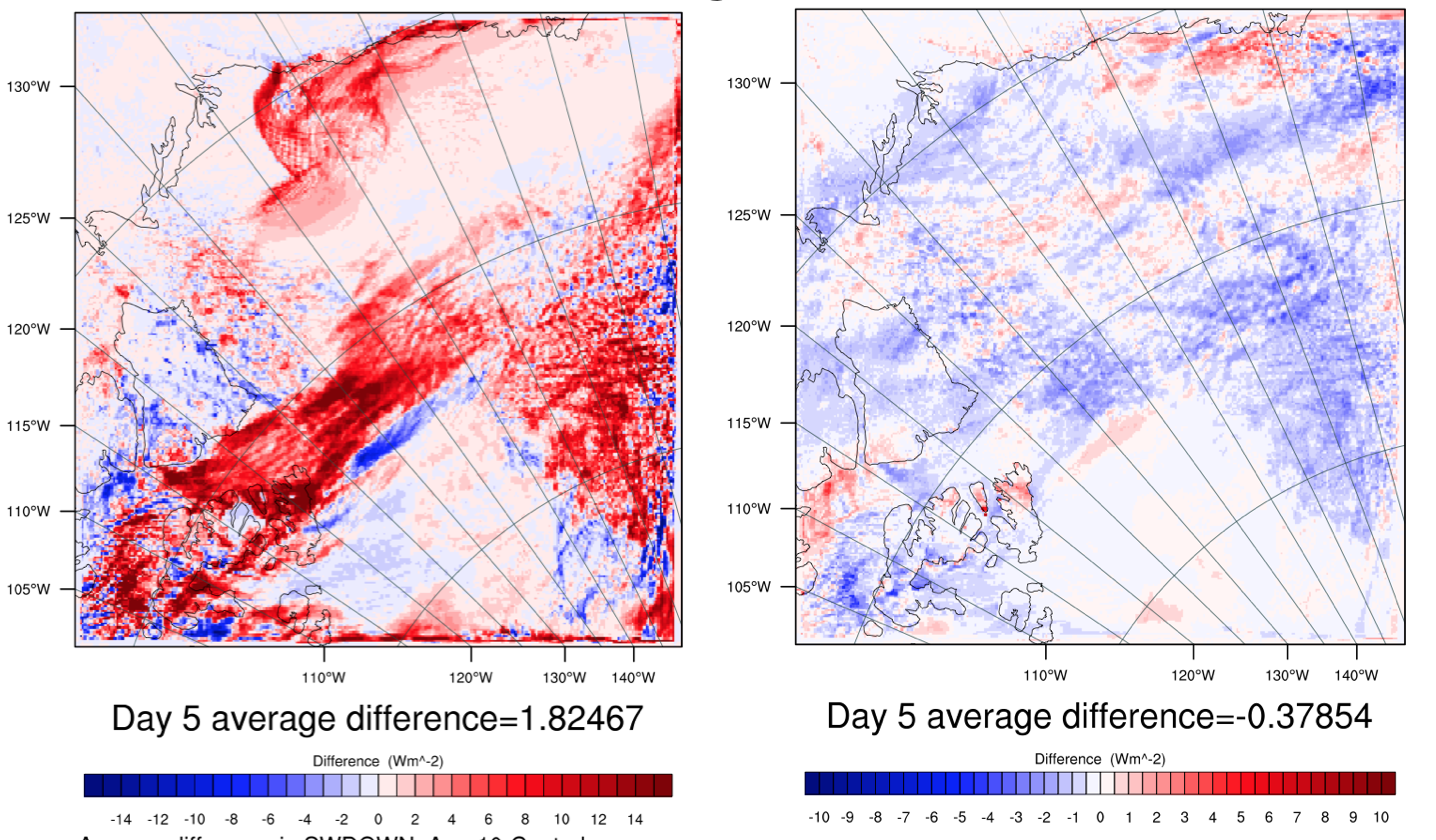
\includegraphics[width=\textwidth]{results/diff_lwupdown_Aero10_Day5.png}
\caption{The average difference in LW downward at the surface and upward at TOA on day 5, from left to right. (preliminary figure)}
\label{fig:lwup_down_r3Day5}
\end{figure}

The area with lack of change in LW up or down is approximately the same area as where there is a negative change in LH and SH upward from the surface over the sea ice, see figure~\ref{fig:lhhfx_r3Day5}. Since there has been no change in LW there is no loss of warming from a decrease in LW reaching the surface, but the change can possibly be explained by looking at the SW radiation. The downward SW at the surface has been significantly decreased as a consequence of the increase in aerosol number concentration, see figure~\ref{fig:swup_down_r3Day5}. The SW radiation has been reflected by the smaller and more numerous droplets. This is known as the Twomey effect, and was described in Chapter~\ref{chap:theory}. 

\begin{figure}[h!]
\centering
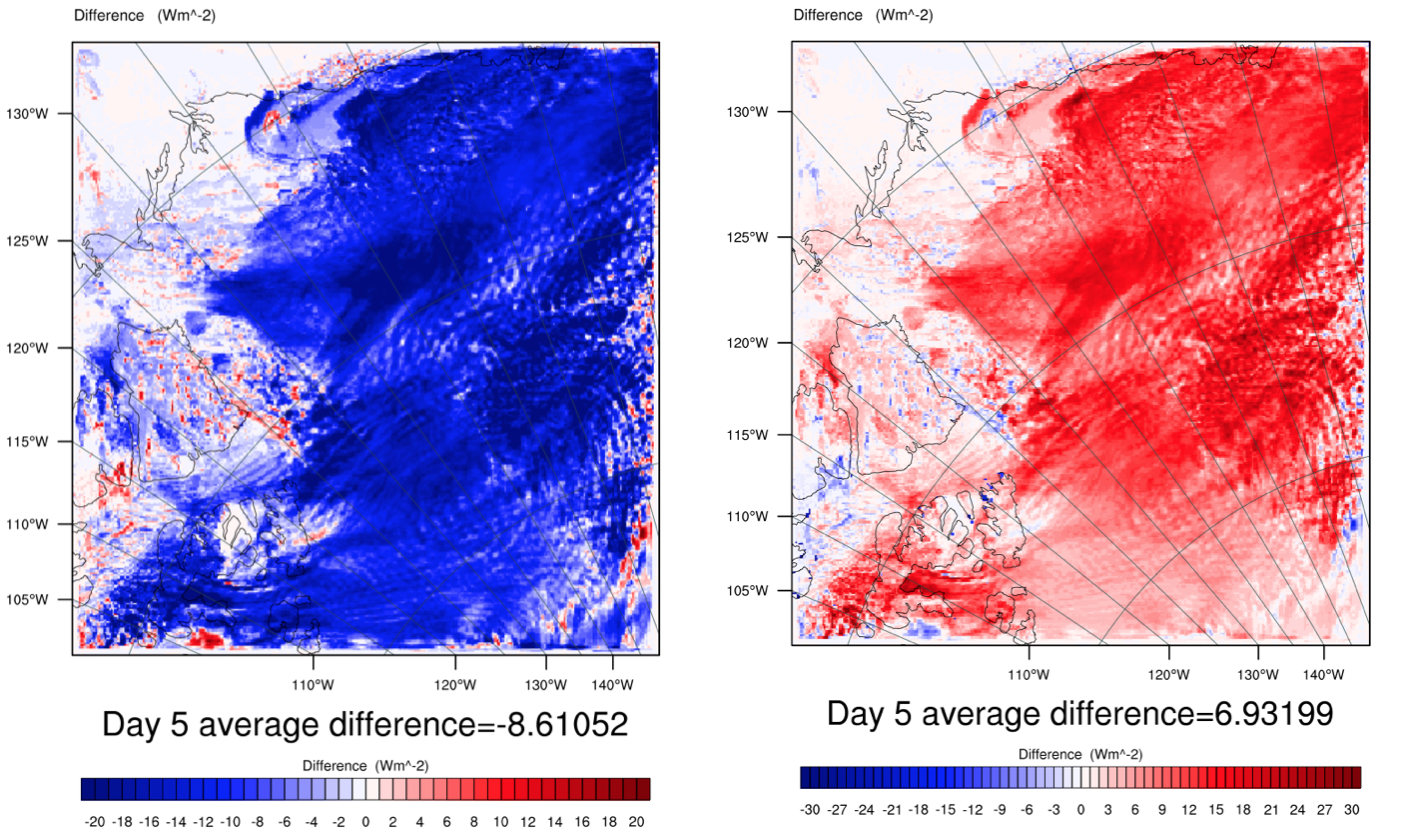
\includegraphics[width=0.9\textwidth]{results/diff_swupdown_Aero10_Day5.png}
\caption{The average difference in SW downward at the surface, and upward on TOA at day 5, from left to right. (preliminary figure)}
\label{fig:swup_down_r3Day5}
\end{figure}

\begin{figure}[h!]
\centering
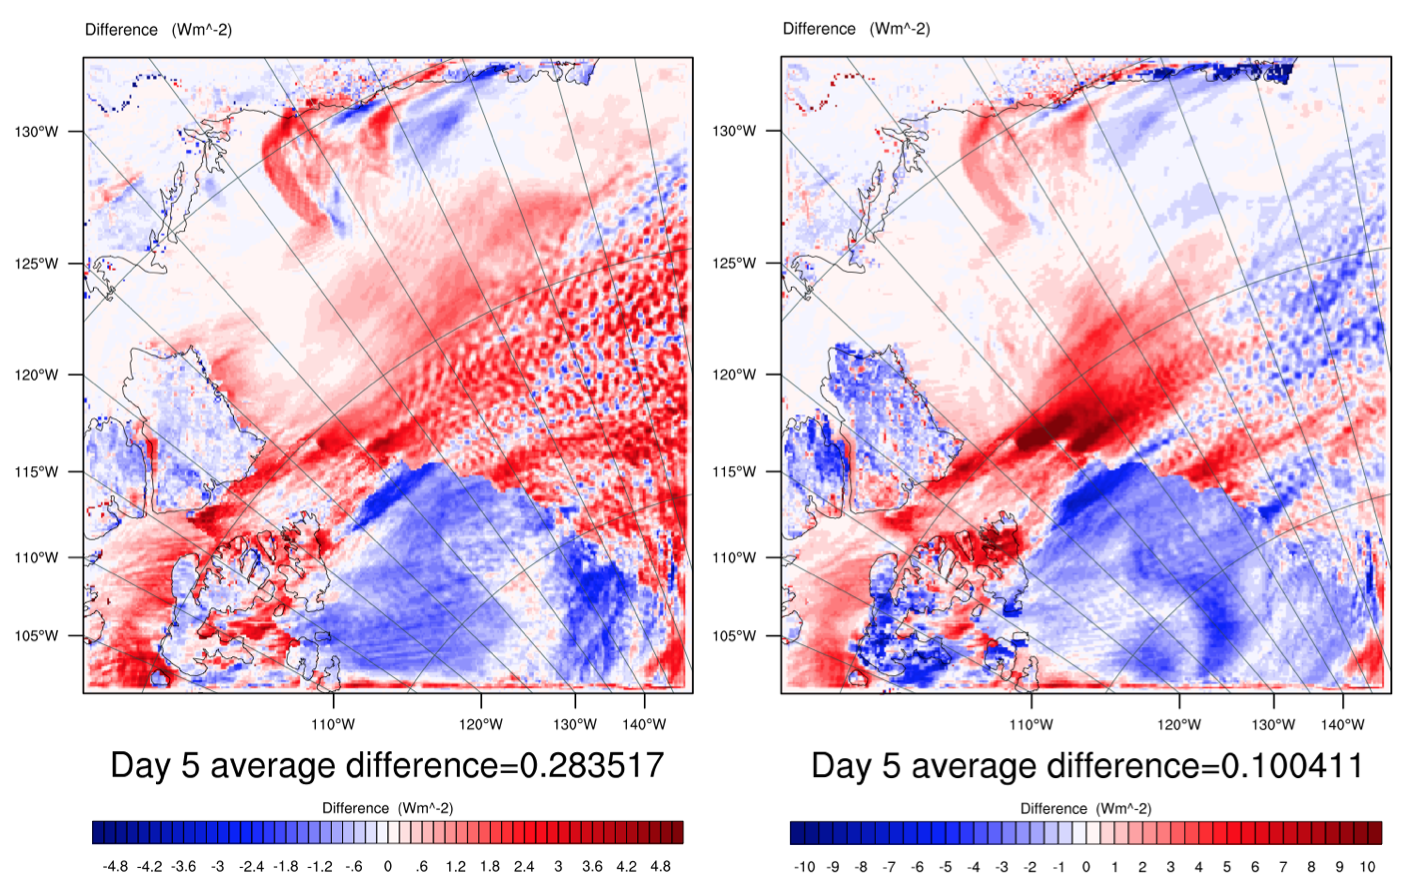
\includegraphics[width=0.9\textwidth]{results/diff_lhhfx_Aero10_Day5.png}
\caption{The average difference in LH and SH upward at the surface on day 5, from left to right. (preliminary figure)}
\label{fig:lhhfx_r3Day5}
\end{figure}

\begin{figure}[h!]
\centering
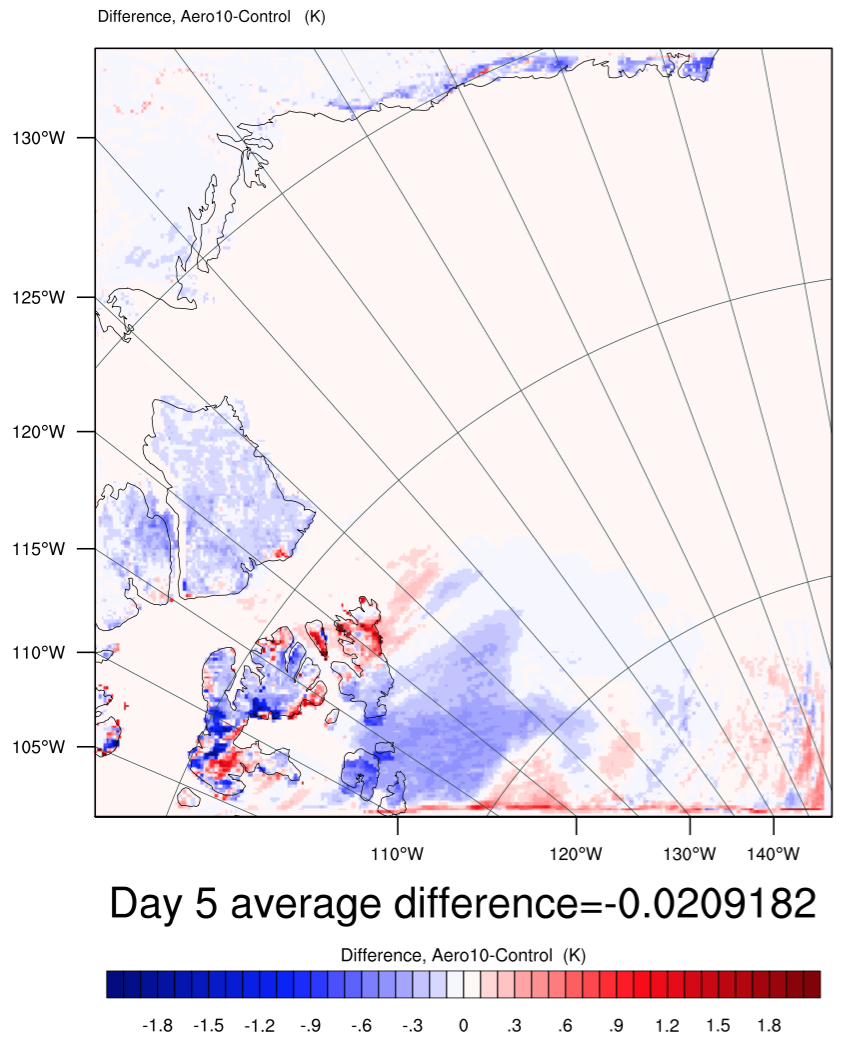
\includegraphics[width=0.5\textwidth]{results/diff_skintemp_Aero10_Day5.png}
\caption{The average difference in skin temperature (the temperature of the surface), for day 5.}
\label{fig:skintemp_r3Day5}
\end{figure}
The albedo of sea ice is typically 0.5-0.7 which means that a fraction of the incident SW radiation is absorbed. Since the amount of incident SW radiation at the surface has been reduced by the cloud cover, the absorbed radiation is less than for a higher incident amount. The ice therefore has a lower temperature to give off SH with. 

%Look at temperature changes at the surface. Over ice and ocean.. 
The skin temperature, figure~\ref{fig:skintemp_r3Day5}, for the domain shows a small decrease in the same area as where there is less sensible and latent heat release.

Also the dynamics over ice and the ocean are different, so this could have an effect. The cold air over the ice may be intensified, while the sea surface temperature (SST) is the same for all the runs and there is no coupling with the ocean. There will therefore be no changes in the SSTs that could have an effect on the dynamics over the ocean. So the response may be smaller there...?


%Her kan det være interessant å se på\\
%Differanser i\\
%- SW fluks\\
%- LW fluks\\
%- LH \\
%- SH, følbar varme... har jeg det?\\
%- Dråpestørrelse\\
%- Skyvannmengde\\

%Må få laget disse figurene sånn at Jon Egill og Kari kan se på dem, og sånn at jeg kan tenke på dem og reflektere og diskutere med meg selv!

%Må ha skala på labelbar som gjør det leselig, og som fremhever de små forskjellene -- for de kan ha stor betydning..!

% Må også oppgi gjennomsnittsverdi for hele feltet (for å hjelpe leseren) of minimums og maksimumsverdiene, siden de ikke er med på labal baren.

%Hvordan de forskjellige tingene påvirker hverandre må være dekket i teorien.!

%Jon Egill har avtalt eksamen 19. juni. Erik Berge er sensor! Hvem er intern?
